
\documentclass[11pt,a4paper]{article}

\usepackage[utf8]{inputenc}
\usepackage[T1]{fontenc}
\usepackage[spanish,es-tabla]{babel}
\usepackage{lmodern}
\usepackage[a4paper,margin=2.35cm]{geometry}
\usepackage{graphicx}
\usepackage{booktabs}
\usepackage{array}
\usepackage{float}
\usepackage{caption}
\usepackage{hyperref}
\usepackage{xcolor}
\usepackage{setspace}
\usepackage{enumitem}
\usepackage{multirow}

\graphicspath{{codigo/outputs/figures/}}

\hypersetup{
    colorlinks=true,
    linkcolor=blue,
    urlcolor=blue,
    citecolor=blue,
    pdftitle={Generación y validación de datos sintéticos},
    pdfauthor={Laura Cabaleiro Pintos; Marcelo Ferreiro Sánchez}
}

\setstretch{1.08}
\setlength{\parskip}{0.42em}
\setlength{\parindent}{0pt}

\title{\textbf{Generación y validación de datos sintéticos}\\
\large Dataset médico tabular: Breast Cancer Wisconsin (Diagnostic)}
\author{Laura Cabaleiro Pintos \\ Marcelo Ferreiro Sánchez}
\date{\today}

\begin{document}
\maketitle
\thispagestyle{empty}

\section{Introducción}

La generación de datos sintéticos resulta especialmente útil en biomedicina porque permite compartir, explorar y prototipar modelos sobre conjuntos artificiales sin exponer directamente los registros originales. Sin embargo, un conjunto sintético no debe juzgarse solo por su parecido superficial con el real. Para que su uso sea razonable, debe conservar propiedades estadísticas relevantes, mantener la señal necesaria para tareas analíticas y, al mismo tiempo, no revelar individuos concretos del entrenamiento.

En este trabajo se aborda ese problema sobre un dataset médico tabular público mediante una estrategia generativa basada en \textit{Gaussian Mixture Models} (GMM) condicionales por clase. El objetivo no es únicamente generar observaciones artificiales, sino validar si el conjunto resultante es suficientemente \textbf{fiel}, \textbf{útil} y \textbf{seguro}. Para reforzar la solidez del análisis, además de un experimento \textit{holdout} clásico, se añade validación cruzada estratificada de 5 \textit{folds} y una evaluación adicional de privacidad mediante un ataque simple de \textit{membership inference}.

\section{Descripción del dataset y estrategia empleada}

El conjunto empleado es \textit{Breast Cancer Wisconsin (Diagnostic)}, un dataset médico tabular público disponible en el repositorio de la UCI. Se trata de un problema de clasificación binaria orientado al diagnóstico de lesiones mamarias a partir de medidas continuas extraídas de imágenes de aspirado con aguja fina. Contiene 569 observaciones y 30 variables numéricas.

Este dataset resulta adecuado para una práctica de síntesis tabular por tres motivos. Primero, pertenece al dominio médico, alineándose con el enunciado. Segundo, combina una tarea clínica bien definida con variables continuas relativamente limpias, lo que facilita el análisis de fidelidad estadística. Tercero, su tamaño moderado permite estudiar el compromiso entre fidelidad, utilidad y privacidad sin introducir una complejidad computacional innecesaria.

\begin{table}[H]
\centering
\renewcommand{\arraystretch}{1.2}
\begin{tabular}{>{\raggedright\arraybackslash}p{4.9cm} p{9.6cm}}
\toprule
\textbf{Elemento} & \textbf{Descripción} \\
\midrule
Enlace al dataset público & \url{https://archive.ics.uci.edu/dataset/17/breast+cancer+wisconsin+diagnostic} \\
Estrategia de generación & GMM condicionales por clase (una mezcla por etiqueta diagnóstica) \\
Librería empleada & \url{https://scikit-learn.org/stable/modules/generated/sklearn.mixture.GaussianMixture.html} \\
Tamaño del dataset & 569 filas y 30 variables continuas \\
Protocolo principal & \textit{Holdout} estratificado: 455 train real, 114 test real y 455 muestras sintéticas \\
Validación adicional & Validación cruzada estratificada de 5 \textit{folds} sobre el mismo dataset \\
\bottomrule
\end{tabular}
\caption{Resumen del dataset, la estrategia de generación y el protocolo experimental.}
\end{table}

La estrategia de síntesis es \textit{class-conditional}. En lugar de ajustar un único modelo generativo a todo el dataset, las muestras se separan por diagnóstico y se entrena un GMM independiente para cada clase. Después se generan nuevas muestras sintéticas respetando la proporción original de clases. Este diseño es razonable porque la distribución de cada grupo diagnóstico no tiene por qué ser la misma, y forzar un único generador global puede difuminar la frontera discriminativa relevante para la tarea clínica.

El procedimiento seguido fue:
\begin{itemize}[leftmargin=1.1cm]
    \item escalado estándar usando únicamente el train real de cada experimento;
    \item selección por BIC tanto del número de componentes como del tipo de covarianza, evaluando entre 1 y 6 componentes por clase y comparando configuraciones \texttt{diag} y \texttt{full};
    \item uso de \texttt{n\_init=10} para reducir la sensibilidad a óptimos locales pobres durante el ajuste de los GMM;
    \item generación de un conjunto sintético del mismo tamaño que el train real correspondiente;
    \item recorte final de los valores generados al rango observado en entrenamiento para evitar medidas biomédicas implausibles.
\end{itemize}

En el experimento \textit{holdout}, el BIC seleccionó 1 componente con covarianza \texttt{full} para la clase 0 y 2 componentes con covarianza \texttt{full} para la clase 1.

\begin{figure}[H]
    \centering
    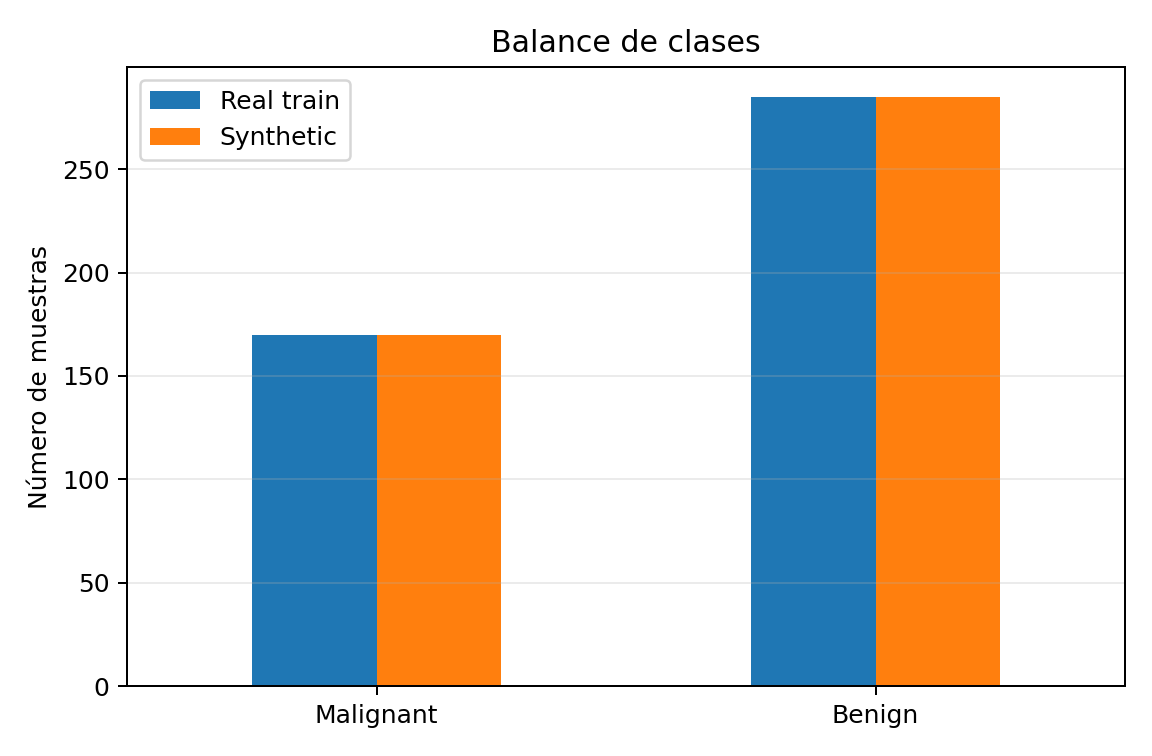
\includegraphics[width=0.70\textwidth]{class_balance.png}
    \caption{El conjunto sintético preserva exactamente el balance de clases del train real.}
\end{figure}

\section{Protocolo experimental}

Para evitar fugas de información, todas las transformaciones y todos los modelos se ajustan exclusivamente sobre el train real de cada partición. En cada \textit{fold}, el escalado, el ajuste del generador, la creación de datos sintéticos y la evaluación posterior se realizan solo con la información disponible en el train de ese \textit{fold}; el test real correspondiente se reserva únicamente para evaluación.

Se utilizaron dos niveles de validación:
\begin{itemize}[leftmargin=1.1cm]
    \item \textbf{Experimento holdout}: permite obtener figuras interpretables y una lectura clara del comportamiento del generador sobre una partición fija.
    \item \textbf{Validación cruzada estratificada de 5 folds}: aporta una estimación más robusta de la estabilidad de las métricas de fidelidad, utilidad y privacidad.
\end{itemize}

La utilidad se midió mediante el protocolo \textbf{TRTR/TSTR}. En TRTR se entrena un clasificador con datos reales y se evalúa en test real; en TSTR se entrena con datos sintéticos y se evalúa en ese mismo test real. Si el rendimiento TSTR permanece cerca del TRTR, puede interpretarse que el conjunto sintético conserva la señal discriminativa relevante.

Los modelos supervisados empleados fueron una regresión logística y un \textit{random forest} con 500 árboles. Esta configuración del bosque reduce la varianza de la evaluación frente a versiones muy pequeñas del modelo y hace más estable la comparación entre entrenamiento con datos reales y con datos sintéticos.

\section{Fidelidad}

La fidelidad se evaluó combinando medidas univariantes y multivariantes. A nivel univariante se compararon medias, desviaciones típicas, estadísticos de Kolmogorov--Smirnov y distancia de Wasserstein normalizada. A nivel multivariante se utilizó la diferencia media absoluta entre matrices de correlación. Esta combinación permite detectar tanto cambios en la forma marginal de cada variable como pérdidas de dependencia entre atributos.

\subsection*{Métricas empleadas}
\begin{table}[H]
\centering
\small
\renewcommand{\arraystretch}{1.2}
\begin{tabular}{p{7.4cm}cc}
\toprule
\textbf{Métrica} & \textbf{Holdout} & \textbf{CV 5-folds (media $\pm$ sd)} \\
\midrule
Diferencia media de medias (unidades z) & 0.029 & 0.028 $\pm$ 0.008 \\
Desviación media del ratio de desviaciones típicas & 0.034 & 0.030 $\pm$ 0.005 \\
KS medio & 0.065 & 0.064 $\pm$ 0.004 \\
KS máximo & 0.165 & 0.118 $\pm$ 0.019 \\
Wasserstein normalizado medio & 0.098 & 0.100 $\pm$ 0.006 \\
Brecha media de correlación & 0.027 & 0.028 $\pm$ 0.002 \\
\bottomrule
\end{tabular}
\end{table}

\subsection*{Discusión de resultados}
Los resultados muestran una fidelidad global buena y, además, estable entre particiones. Las medias sintéticas apenas se desplazan respecto a las reales y tanto el KS medio como la distancia de Wasserstein normalizada permanecen bajos. Esto indica que el generador reproduce razonablemente bien las distribuciones marginales del dataset.

La parte más exigente aparece en la estructura multivariante. Aunque la brecha media de correlación sigue siendo moderada, no es nula. Esto es coherente con la propia naturaleza del enfoque: incluso permitiendo que el BIC seleccione entre covarianza diagonal o completa, el generador sigue siendo un baseline de mezcla gaussiana relativamente simple, que reproduce bien la forma general de los datos pero tiende a suavizar dependencias finas entre atributos. Por tanto, la fidelidad alcanzada es suficiente para análisis exploratorio y experimentación, aunque no equivale a una réplica perfecta del conjunto real.

\begin{figure}[H]
    \centering
    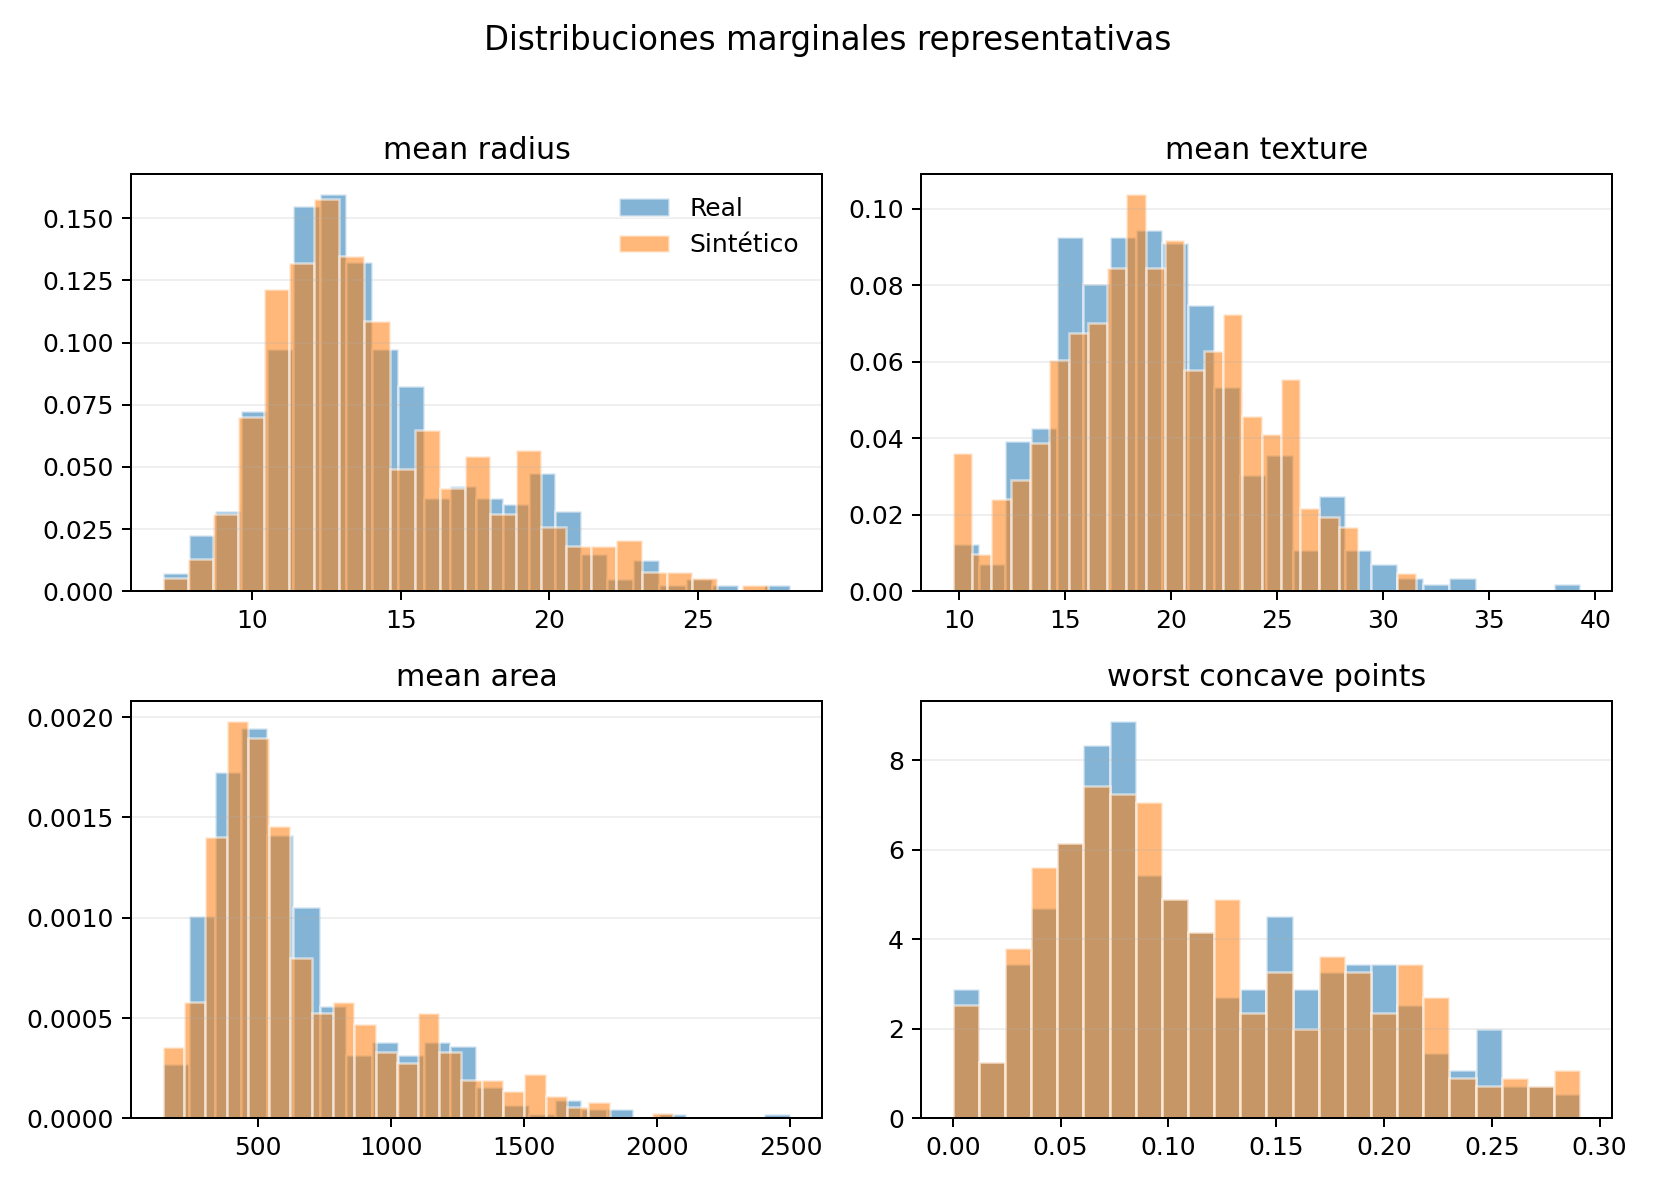
\includegraphics[width=0.90\textwidth]{feature_distributions.png}
    \caption{Distribuciones marginales de cuatro variables representativas en train real y sintético.}
\end{figure}

\begin{figure}[H]
    \centering
    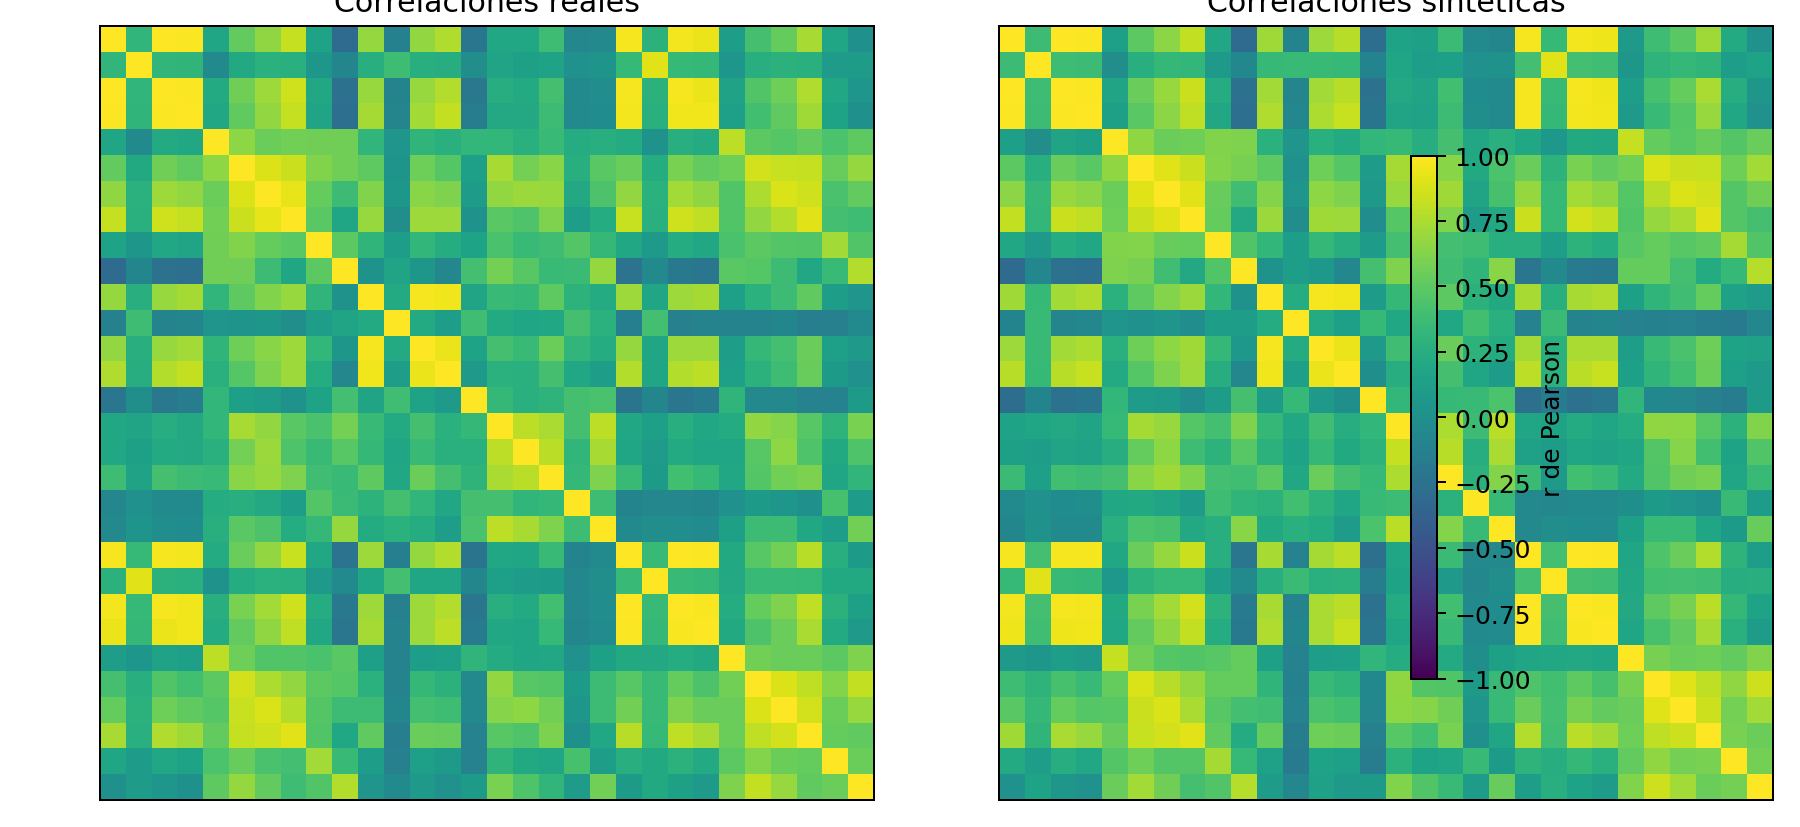
\includegraphics[width=0.88\textwidth]{correlation_heatmaps.png}
    \caption{Estructura de correlaciones en los datos reales y sintéticos.}
\end{figure}

\begin{figure}[H]
    \centering
    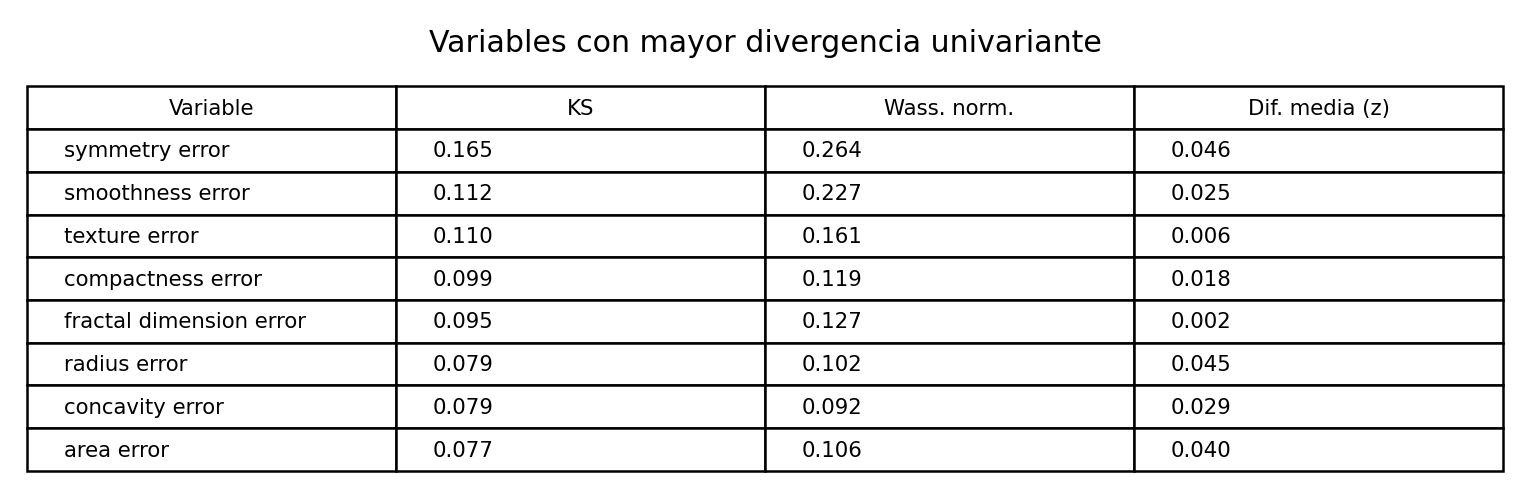
\includegraphics[width=0.88\textwidth]{fidelity_table.png}
    \caption{Variables con mayor divergencia univariante según KS y Wasserstein normalizado.}
\end{figure}

\section{Utilidad}

La utilidad se analizó con el protocolo TRTR/TSTR usando dos modelos supervisados: regresión logística y \textit{random forest}. En ambos casos la evaluación se realiza siempre sobre test real. Esto permite responder a la pregunta relevante para la práctica: \textit{¿sirven los datos sintéticos para entrenar modelos que generalicen sobre datos reales?}

\subsection*{Métricas empleadas}
\begin{table}[H]
\centering
\small
\renewcommand{\arraystretch}{1.2}
\begin{tabular}{lccc}
\toprule
\textbf{Modelo} & \textbf{Accuracy CV (\%)} & \textbf{F1 CV} & \textbf{ROC-AUC CV} \\
\midrule
Logistic Regression (TRTR) & 97.37 $\pm$ 1.86 & 0.979 $\pm$ 0.014 & 0.995 $\pm$ 0.006 \\
Logistic Regression (TSTR) & 97.72 $\pm$ 1.59 & 0.982 $\pm$ 0.012 & 0.996 $\pm$ 0.004 \\
Random Forest (TRTR) & 95.08 $\pm$ 1.59 & 0.961 $\pm$ 0.012 & 0.990 $\pm$ 0.009 \\
Random Forest (TSTR) & 95.26 $\pm$ 0.78 & 0.962 $\pm$ 0.006 & 0.992 $\pm$ 0.006 \\
\bottomrule
\end{tabular}
\end{table}

\subsection*{Discusión de resultados}
La utilidad obtenida es alta. En validación cruzada, los modelos entrenados con datos sintéticos mantienen un rendimiento muy cercano al de los modelos entrenados con datos reales tanto en \textit{accuracy} como en F1 y ROC-AUC. En regresión logística, TSTR incluso queda prácticamente al nivel de TRTR; en \textit{random forest} la diferencia también es pequeña pese a usar una configuración más estable del bosque. Esto sugiere que la señal clínica relevante para clasificar lesiones benignas y malignas se conserva de forma notable.

Además, en el experimento \textit{holdout} el \textit{random forest} mantiene una coincidencia de 10 de las 10 variables más importantes entre entrenamiento real y sintético. Ese dato refuerza la interpretación de que el generador no solo preserva el rendimiento agregado, sino también buena parte de la estructura de señal que el modelo utiliza para decidir. En otras palabras, los datos sintéticos parecen útiles no únicamente porque ``se parezcan'' a los reales, sino porque siguen codificando relaciones predictivas relevantes.

\begin{figure}[H]
    \centering
    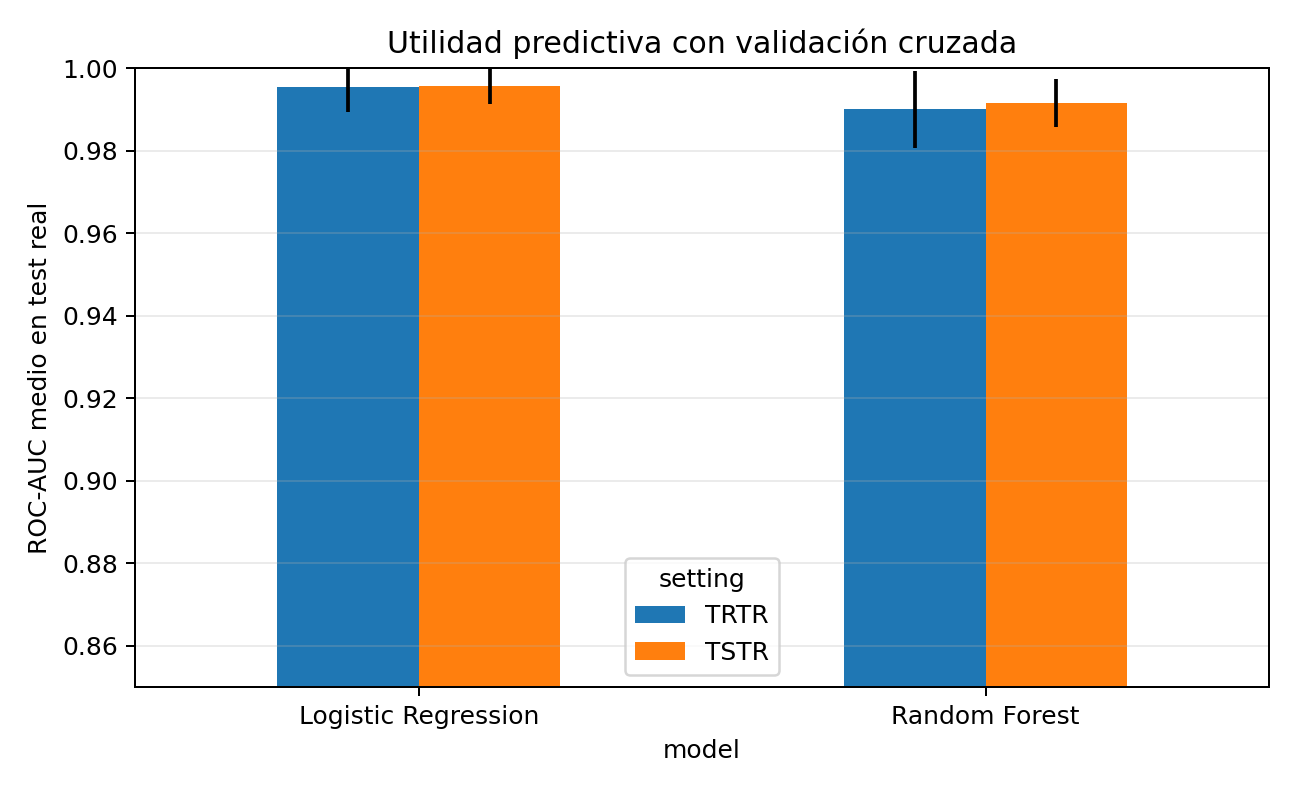
\includegraphics[width=0.80\textwidth]{utility_roc_auc_cv.png}
    \caption{Rendimiento predictivo medio en validación cruzada sobre test real.}
\end{figure}

\section{Privacidad}

La privacidad se estudió desde dos perspectivas complementarias. La primera busca detectar \textbf{copias o vecinos excesivamente cercanos} mediante DCR, NNDR y duplicados exactos. La segunda incorpora un \textbf{ataque simple de membership inference}. En este ataque, el adversario solo observa el conjunto sintético publicado y, para cada registro candidato, calcula su distancia al sintético más cercano. Si los ejemplos de entrenamiento fuesen claramente más cercanos al conjunto sintético que los ejemplos no vistos, el atacante podría inferir membresía con ventaja apreciable.

\subsection*{Métricas empleadas}
\begin{table}[H]
\centering
\small
\renewcommand{\arraystretch}{1.2}
\begin{tabular}{p{7.2cm}cc}
\toprule
\textbf{Indicador} & \textbf{Holdout} & \textbf{CV 5-folds (media $\pm$ sd)} \\
\midrule
Tasa de duplicados exactos & 0.00\% & 0.00 $\pm$ 0.00 \\
DCR mediano sintético $\rightarrow$ train & 2.376 & 2.413 $\pm$ 0.044 \\
DCR mediano test real $\rightarrow$ train & 2.102 & 2.156 $\pm$ 0.079 \\
NNDR mediano sintético & 0.934 & 0.932 $\pm$ 0.005 \\
\% sintéticos por debajo del p1 del DCR del test & 0.00\% & 0.92 $\pm$ 0.99 \\
\% sintéticos por debajo del p5 del DCR del test & 0.66\% & 2.90 $\pm$ 1.82 \\
AUC del ataque de membership & 0.511 & 0.525 $\pm$ 0.028 \\
Ventaja máxima del atacante & 0.060 & 0.079 $\pm$ 0.029 \\
Balanced accuracy óptima del atacante & 0.530 & 0.540 $\pm$ 0.014 \\
\bottomrule
\end{tabular}
\end{table}

\subsection*{Discusión de resultados}
Los indicadores de proximidad son tranquilizadores. No aparecen duplicados exactos y el DCR mediano de los sintéticos es superior al del test real independiente, lo que reduce la sospecha de copia directa. Además, solo una fracción muy pequeña de los registros sintéticos cae por debajo del percentil 5 del DCR del test real y ninguno queda por debajo del percentil 1. El NNDR mediano cercano a 1 sugiere que, cuando existe un vecino cercano, no suele tratarse de una coincidencia aislada extrema sino de regiones del espacio con varios puntos plausibles.

El ataque de \textit{membership inference} aporta una comprobación más exigente. Un AUC de 0.511 en holdout y de 0.525 $\pm$ 0.028 en validación cruzada está cerca del azar, y la \textit{balanced accuracy} óptima del atacante apenas supera 0.540. Esto no demuestra privacidad formal, pero sí indica que la publicación del conjunto sintético no ofrece una señal fuerte para distinguir de forma fiable entre ejemplos pertenecientes al train y ejemplos no vistos. En consecuencia, el riesgo de memorización parece bajo en este experimento.

Aun así, conviene ser prudentes. Esta evaluación sigue siendo empírica y específica del ataque considerado. No equivale a una garantía de privacidad diferencial ni descarta ataques más sofisticados. Lo correcto es interpretar los resultados como evidencia de \textbf{ausencia de copia evidente} y \textbf{baja capacidad de inferencia de membresía} en el escenario analizado.

\begin{figure}[H]
    \centering
    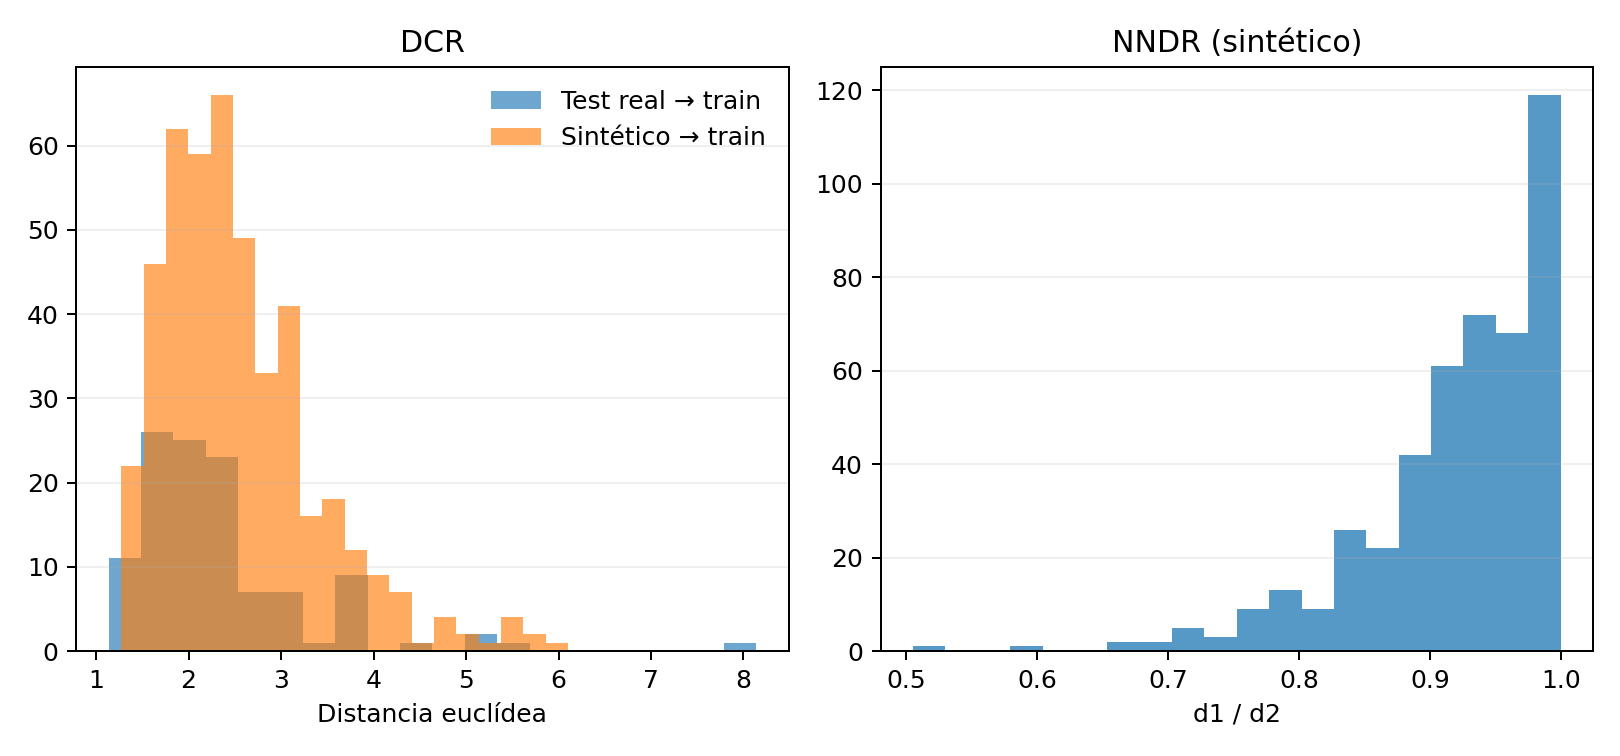
\includegraphics[width=0.88\textwidth]{privacy_dcr_nndr.png}
    \caption{Comparativa de DCR y distribución de NNDR en el conjunto sintético.}
\end{figure}

\begin{figure}[H]
    \centering
    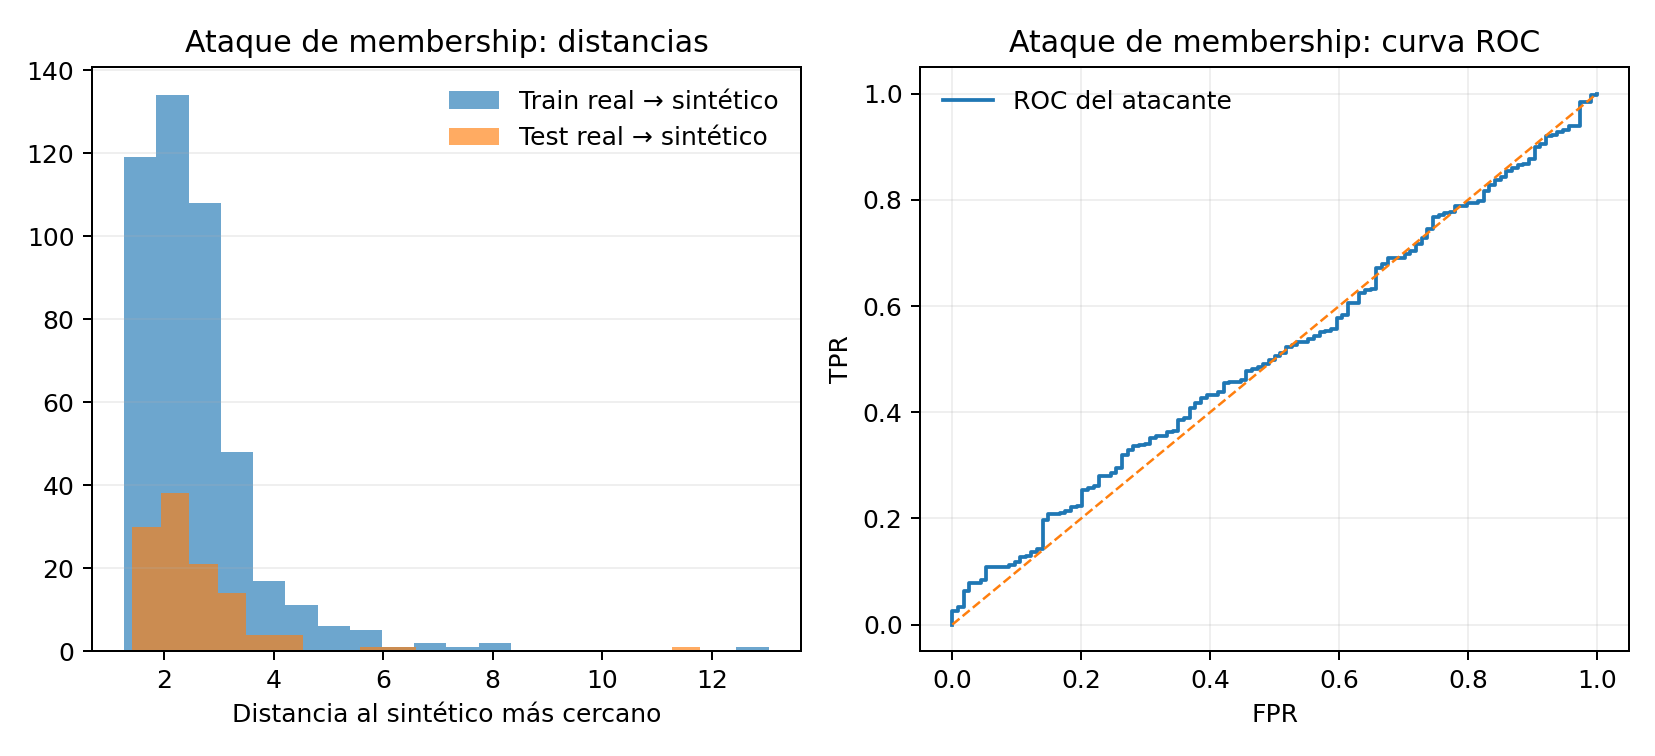
\includegraphics[width=0.88\textwidth]{privacy_membership_attack.png}
    \caption{Ataque simple de \textit{membership inference}: distancias a sintéticos y curva ROC del atacante.}
\end{figure}

\section{Conclusión}

La estrategia basada en \textit{Gaussian Mixture Models} condicionales por clase ofrece un compromiso sólido entre fidelidad, utilidad y privacidad para este dataset médico tabular. La fidelidad es buena en términos de distribuciones marginales y razonable en estructura multivariante; la utilidad predictiva se mantiene alta incluso cuando los modelos se entrenan solo con datos sintéticos; y la evaluación de privacidad no muestra señales claras de copia ni de inferencia de membresía fuerte.

El principal límite del enfoque está en su simplicidad relativa frente a librerías especializadas de síntesis tabular. Aun así, el baseline se ha reforzado seleccionando por BIC tanto el número de componentes como el tipo de covarianza, ampliando la búsqueda hasta 6 componentes por clase y utilizando \texttt{n\_init=10} para estabilizar el ajuste. Incluso con esas mejoras, el generador sigue tendiendo a suavizar parte de las dependencias finas entre variables; sin embargo, esa misma sencillez también contribuye a un comportamiento estable, reproducible y fácil de interpretar. Como trabajo futuro, sería interesante comparar este baseline con librerías especializadas como SDV, Synthcity o BeGREAT y ampliar la sección de privacidad con ataques más agresivos o mecanismos formales de protección.

\end{document}
